

% Default to the notebook output style


% Inherit from the specified cell style.




    
\documentclass{article}

    
    
    \usepackage{graphicx} % Used to insert images
    \usepackage{adjustbox} % Used to constrain images to a maximum size 
    \usepackage{color} % Allow colors to be defined
    \usepackage{enumerate} % Needed for markdown enumerations to work
    \usepackage{geometry} % Used to adjust the document margins
    \usepackage{amsmath} % Equations
    \usepackage{amssymb} % Equations
    \usepackage[mathletters]{ucs} % Extended unicode (utf-8) support
    \usepackage[utf8x]{inputenc} % Allow utf-8 characters in the tex document
    \usepackage{fancyvrb} % verbatim replacement that allows latex
    \usepackage{grffile} % extends the file name processing of package graphics 
                         % to support a larger range 
    % The hyperref package gives us a pdf with properly built
    % internal navigation ('pdf bookmarks' for the table of contents,
    % internal cross-reference links, web links for URLs, etc.)
    \usepackage{hyperref}
    \usepackage{longtable} % longtable support required by pandoc >1.10
    

    
    \definecolor{orange}{cmyk}{0,0.4,0.8,0.2}
    \definecolor{darkorange}{rgb}{.71,0.21,0.01}
    \definecolor{darkgreen}{rgb}{.12,.54,.11}
    \definecolor{myteal}{rgb}{.26, .44, .56}
    \definecolor{gray}{gray}{0.45}
    \definecolor{lightgray}{gray}{.95}
    \definecolor{mediumgray}{gray}{.8}
    \definecolor{inputbackground}{rgb}{.95, .95, .85}
    \definecolor{outputbackground}{rgb}{.95, .95, .95}
    \definecolor{traceback}{rgb}{1, .95, .95}
    % ansi colors
    \definecolor{red}{rgb}{.6,0,0}
    \definecolor{green}{rgb}{0,.65,0}
    \definecolor{brown}{rgb}{0.6,0.6,0}
    \definecolor{blue}{rgb}{0,.145,.698}
    \definecolor{purple}{rgb}{.698,.145,.698}
    \definecolor{cyan}{rgb}{0,.698,.698}
    \definecolor{lightgray}{gray}{0.5}
    
    % bright ansi colors
    \definecolor{darkgray}{gray}{0.25}
    \definecolor{lightred}{rgb}{1.0,0.39,0.28}
    \definecolor{lightgreen}{rgb}{0.48,0.99,0.0}
    \definecolor{lightblue}{rgb}{0.53,0.81,0.92}
    \definecolor{lightpurple}{rgb}{0.87,0.63,0.87}
    \definecolor{lightcyan}{rgb}{0.5,1.0,0.83}
    
    % commands and environments needed by pandoc snippets
    % extracted from the output of `pandoc -s`
    \DefineVerbatimEnvironment{Highlighting}{Verbatim}{commandchars=\\\{\}}
    % Add ',fontsize=\small' for more characters per line
    \newenvironment{Shaded}{}{}
    \newcommand{\KeywordTok}[1]{\textcolor[rgb]{0.00,0.44,0.13}{\textbf{{#1}}}}
    \newcommand{\DataTypeTok}[1]{\textcolor[rgb]{0.56,0.13,0.00}{{#1}}}
    \newcommand{\DecValTok}[1]{\textcolor[rgb]{0.25,0.63,0.44}{{#1}}}
    \newcommand{\BaseNTok}[1]{\textcolor[rgb]{0.25,0.63,0.44}{{#1}}}
    \newcommand{\FloatTok}[1]{\textcolor[rgb]{0.25,0.63,0.44}{{#1}}}
    \newcommand{\CharTok}[1]{\textcolor[rgb]{0.25,0.44,0.63}{{#1}}}
    \newcommand{\StringTok}[1]{\textcolor[rgb]{0.25,0.44,0.63}{{#1}}}
    \newcommand{\CommentTok}[1]{\textcolor[rgb]{0.38,0.63,0.69}{\textit{{#1}}}}
    \newcommand{\OtherTok}[1]{\textcolor[rgb]{0.00,0.44,0.13}{{#1}}}
    \newcommand{\AlertTok}[1]{\textcolor[rgb]{1.00,0.00,0.00}{\textbf{{#1}}}}
    \newcommand{\FunctionTok}[1]{\textcolor[rgb]{0.02,0.16,0.49}{{#1}}}
    \newcommand{\RegionMarkerTok}[1]{{#1}}
    \newcommand{\ErrorTok}[1]{\textcolor[rgb]{1.00,0.00,0.00}{\textbf{{#1}}}}
    \newcommand{\NormalTok}[1]{{#1}}
    
    % Define a nice break command that doesn't care if a line doesn't already
    % exist.
    \def\br{\hspace*{\fill} \\* }
    % Math Jax compatability definitions
    \def\gt{>}
    \def\lt{<}
    % Document parameters
    \title{Circuitos usando Diodos}
    
    
    

    
    % Prevent overflowing lines due to hard-to-break entities
    \sloppy 
    % Setup hyperref package
    \hypersetup{
      breaklinks=true,  % so long urls are correctly broken across lines
      colorlinks=true,
      urlcolor=blue,
      linkcolor=darkorange,
      citecolor=darkgreen,
      }
    % Slightly bigger margins than the latex defaults
    
    \geometry{verbose,tmargin=1in,bmargin=1in,lmargin=1in,rmargin=1in}
    
    

    \begin{document}
    
    
    \maketitle
    
    

    
    \section{Curvas Caracteristicas}\label{curvas-caracteristicas}

Con un circuito simple se puede utilizar el circuito que se muestra
acontinuación:

\begin{figure}[htbp]
\centering
\includegraphics{images/curvadiodocir.png}
\caption{Circuito Básico}
\end{figure}

dado que la fuente de corriente puede tener cualquier valor de voltaje
(teoricamente), si controlamos la corriente $I_{D}$ entonces obtendremos
una variación en el voltaje del diodo $V_{D}$, la cual debe de ser
similar al expresado por la expresión:

\begin{equation}\label{eq:diodo}
I_{D}=I_{s}\left( e^{\frac{V_{D}}{nV_{T}}}-1\right)
\end{equation}

Utilizando el program LTspice para obtener el comportamiento de
diferentes diodos se obtiene la siguiente gráfica. (Los archivos son:
\href{http://cacie.ens.uabc.mx/~mmiranda/cursos/notas/Electronica/diodos_curva.asc}{diodos\_curvas.asc}
el archivo de LTspice y el de
\href{http://cacie.ens.uabc.mx/~mmiranda/cursos/notas/Electronica/curvasdiodos.txt}{curvasdiodos.txt}
contiene los datos que se usan en el ejemplo.


    \begin{center}
    \adjustimage{max size={0.5\linewidth}{0.5\paperheight}}{Circuitos usando Diodos_files/Circuitos usando Diodos_1_0.png}
    \end{center}
    { \hspace*{\fill} \\}
    
    \section{Circuito Rectificador de media
onda}\label{circuito-rectificador-de-media-onda}

El circuito más simple con un diodo es el conocido como rectificador de
media onda el cual consiste de una fuente de voltaje $V_{i}$, un
resistencia $R$ y un diodo $D$ en seria, como se muestra en la siguiente
figura

\begin{figure}[htbp]
\centering
\includegraphics{images/diodosimple.png}
\caption{Circuito con un diodo}
\end{figure}

Utilizando la ley de Kircchof de voltajes y la ley de Ohm se tiene

\begin{equation}\label{eq:uno}
V_{i}=I_{D}R+V_{D}
\end{equation}

dado que los elementos estan en serie se tiene que corriente es la
misma, por lo tanto es posible encontrar la corriente total con la
expresión para la corriente del diodo

\begin{equation}\label{eq:id}
I_{D}=I_{s}\left( e^{\frac{V_{D}}{nV_{T}}}-1\right)
\end{equation}

sustituyendo \eqref{eq:id} en \eqref{eq:uno}

\begin{equation}\label{eq:dos}
V_{i}=I_{s}\left( e^{\frac{V_{D}}{nV_{T}}}-1\right)R+V_{D}
\end{equation}

La expresión \eqref{eq:dos} es una ecuación trascendente (Una ecuación
trascendente es una igualdad entre dos expresiones matemáticas en las
que aparecen una o más incógnitas relacionadas mediante operaciones
matemáticas, que no son únicamente algebraicas, y cuya solución no puede
obtenerse empleando solo las herramientas propias del álgebra.) lo cual
no permite encontrar una solución analitica.

Para resolver una ecuación trascendente se utilizan dos métodos que son:
por estimación y gráfico.

\subsection{Estimación}\label{estimaciuxf3n}

Considerese una expresión del tipo

\begin{equation}\label{eq:idea1}
y=f(x,p)
\end{equation}

donde $y$ es una salida conocida (Variable dependiente), $x$ es una
entrada (Variable independiente) y $p$ son un conjunto de parámetros. Si
$f(x,p)$ es una ecuación que no tiene solución analitica, entonces no se
puede calcular su solución exacta. Sin embargo, es posible estimar una
solución aproximada $\hat{y}$ con el método de estimación. En este
método se asignan valores a la incognita hasta que el error ($E_{y}$)
entre la solución exacta $y$ y la solución estimada $\hat{y}$ es menor a
un cierto valor establecido. Esto se puede expresar como:

\[
E_{y}=|y-\hat{y}|\leq k
\]

Por lo que este metodo requiere que los coeficientes de la expresión a
evular sea conocidos.

\subsubsection{Ejemplo 1}\label{ejemplo-1}

en el caso de la expresión \eqref{eq:dos} consideramos que $R=2k\Omega$,
$V_{i}=5$, $n=2$, y $V_{T}=26mV$. En la siguiente gráfica se muestra el
valor estimado de la expresión \eqref{eq:dos} al sustituir valores de
los parámetros y considerar $0\leq V_{D} \leq 1$


    \begin{center}
    \adjustimage{max size={0.5\linewidth}{0.5\paperheight}}{Circuitos usando Diodos_files/Circuitos usando Diodos_3_0.png}
    \end{center}
    { \hspace*{\fill} \\}
    
    De la gráfica anterior se observa que para valores de $V_{D}$ mayores a
0.8, la salida estimada es mucho mayor que la salida esperada, por lo
que haciendo una nueva iteración $0\leq V_{D} \leq 0.7$, se obtiene la
siguiente gráfica


    \begin{center}
    \adjustimage{max size={0.5\linewidth}{0.5\paperheight}}{Circuitos usando Diodos_files/Circuitos usando Diodos_5_0.png}
    \end{center}
    { \hspace*{\fill} \\}
    
    De los resultados mostrados en la gráfica anterior se puede concluir que
el valor estimado se aproxima al valor deseado caundo
$0.5\leq V_{D} \leq 0.6$, para realizar una mejor aproximación se
utiliza el error de estimacion

\begin{equation}
E=V_{i}-\hat{V_{i}}
\end{equation}

donde $\hat{V_{i}}$ es el valor estimado a través de la expresion
\eqref{eq:dos}


    \begin{center}
    \adjustimage{max size={0.5\linewidth}{0.5\paperheight}}{Circuitos usando Diodos_files/Circuitos usando Diodos_7_0.png}
    \end{center}
    { \hspace*{\fill} \\}
    
    De la gráfica anterior se observa que el error $E$ es igual a 0 cuando
$0.55 \leq V_{D} \leq 0.56$, por lo que hacuendo una nueva aproximación
es posible encontrar un valor exacto. El siguiente paso es proponer que
el intervalo $0.55 \leq V_{D} \leq 0.56$.


    \begin{center}
    \adjustimage{max size={0.5\linewidth}{0.5\paperheight}}{Circuitos usando Diodos_files/Circuitos usando Diodos_9_0.png}
    \end{center}
    { \hspace*{\fill} \\}
    
    Se observa que el error $E=0$ se encuentra en el intervalo
$0.556 \leq V_{D} \leq 0.557$, para encontrar un error con una buena
presición se tiene que realizar este proceso más iteraciones, en este
caso con ayuda de los \textbf{métodos númericos} se cuenta con
algoritmos que hacen posible el cálculo de estos valores de forma
automatica.

Usando uno de estos metodos (metodo de biseccion) se encuentra que el
valor de $V_{D}$ que produce un $E<1^{-4}$ se tiene que:


    \begin{Verbatim}[commandchars=\\\{\}]
El valor estimado de Vd que soluciona el problema es: 0.5564939428778598
    \end{Verbatim}

    el valor de la corriente del diodo utilizando \eqref{eq:diodo} es
$I_{d}=0.0022217530285451636 \approx 2.22mA$


    
    
    \begin{verbatim}
0.0022217530285451636
    \end{verbatim}

    

    \section{Analisis de DC}\label{analisis-de-dc}

En el caso de un circuito con diodos el sistema se puede analizar en dos
partes, cuando el diodo esta polarizado en directa y cuando esta
polariazado en inversa.

\subsection{Polarización directa}\label{polarizaciuxf3n-directa}

En el caso ideal se tiene que un circuito con un diodo que esta
polarizado en directa el diodo se puede considerar como un interruptor
cerrado, tal como se muestra en la siguiente circuito

\begin{figure}[htbp]
\centering
\includegraphics{images/didodcdirecta.png}
\caption{Circuito con un diodo polarizado en directa}
\end{figure}

donde $V_{d}=0$ y por lo tanto la corriente se obtiene con la expresión

\begin{equation}
I_{d}=\frac{V_{i}}{R}
\end{equation}

Sin embargo, la expresión anterior es incorrecta si consideramos que la
corriente dada en el diodo es determinada por la expresión
\eqref{eq:diodo}. En general del ejemplo anterior se observa que es
dificil calcular el valor de la corriente con las ecuaciones exactas,
por lo que se simplifica el problema que una vez establecida la
corriente de DC, el voltaje del diodo $V_{d}=V_{k}$ donde
$V_{k} \geq 0$, siendo el valor de $V_{k}$ determinado de forma
heuristica en función del tipo de diodo, por lo que una función
aproximada para calcular la corriente sería:

\begin{equation}\label{eq:idaprox}
I_{d}=\frac{V_{i}-V_{k}}{R}
\end{equation}

Si consideramos la expresión \eqref{eq:idaprox} en el ejemplo 1,
considerando que $V_{k}=0.7$ se tiene

\[
I_{d}=\frac{V_{i}-V_{k}}{R}=\frac{(5-0.7)V}{2k \Omega }=2.15mA
\]

lo cual solo tiene un error de $0.08mA$ con respecto al cálculo
utilizando la expresión \eqref{eq:diodo}

\subsection{Polarización inversa}\label{polarizaciuxf3n-inversa}

En el caso de la polarizción inversa se tiene que el diodo se puede
sustituir con un interruptor abierto como se muestra en la figura que
sigue:

\begin{figure}[htbp]
\centering
\includegraphics{images/didodcinversa.png}
\caption{Circuito con un diodo polarizado en inversa}
\end{figure}

en el caso del circuito anterior se tiene que el voltaje en la
resistencia $V_{R}=0$, ya que no fluye corriente alguna, por lo que se
tiene que $V_{d}=V_{i}$. Lo anterior será valido mientras no se alcance
el voltaje de conducción en inversa (Voltaje de avalancha $V_{a}$ o
Voltaje Zenner $V_{z}$), ya que al alcanzar el voltaje de conducción en
inversa el diodo se comporta de forma similar cuando esta polarizado en
directa. Solo que ahora el voltaje utilizado para la expresión
\eqref{eq:idaprox} no es $V_{k}$ sino el voltaje de avalancha $V_{A}$

\begin{equation}\label{eq:idinversaaprox}
I_{d}=\frac{V_{i}-V_{A}}{R}
\end{equation}

    \section{Circuito Rectificador de Onda
Completa}\label{circuito-rectificador-de-onda-completa}

El circuito rectificador de onda completa se muestra en la siguiente
figura.

\begin{figure}[htbp]
\centering
\includegraphics[width=0.5\textwidth]{images/puentededidos.png}
\caption{Rectificador de Onda Completa}
\end{figure}

\subsection{Ciclo positivo}\label{ciclo-positivo}

\begin{figure}[htbp]
\centering
\includegraphics{images/puentediodos2pos.png}
\caption{Rectificador de Onda Completa Ciclo Positivo}
\end{figure}

\subsection{Ciclo negativo}\label{ciclo-negativo}

\begin{figure}[htbp]
\centering
\includegraphics{images/puentediodos2neg.png}
\caption{Rectificador de Onda Completa Ciclo Negativo}
\end{figure}


    \begin{center}
    \adjustimage{max size={0.5\linewidth}{0.5\paperheight}}{Circuitos usando Diodos_files/Circuitos usando Diodos_16_0.png}
    \end{center}
    { \hspace*{\fill} \\}
    
    \section{Fuente de voltaje de CD con
diodos}\label{fuente-de-voltaje-de-cd-con-diodos}

\subsection{Transformador}\label{transformador}

Se denomina transformador a un dispositivo eléctrico que permite
aumentar o disminuir la tensión en un circuito eléctrico de corriente
alterna, manteniendo la potencia. La potencia que ingresa al equipo, en
el caso de un transformador ideal (esto es, sin pérdidas), es igual a la
que se obtiene a la salida. Las máquinas reales presentan un pequeño
porcentaje de pérdidas, dependiendo de su diseño y tamaño, entre otros
factores.

El transformador es un dispositivo que convierte la energía eléctrica
alterna de un cierto nivel de tensión, en energía alterna de otro nivel
de tensión, basándose en el fenómeno de la inducción electromagnética.
Está constituido por dos o más bobinas de material conductor, devanadas
sobre un núcleo cerrado de material ferromagnético, pero aisladas entre
sí eléctricamente. La única conexión entre las bobinas la constituye el
flujo magnético común que se establece en el núcleo. El núcleo,
generalmente, es fabricado bien sea de hierro o de láminas apiladas de
acero eléctrico, aleación apropiada para optimizar el flujo magnético.
Las bobinas o devanados se denominan primario y secundario según
correspondan a la entrada o salida del sistema en cuestión,
respectivamente. También existen transformadores con más devanados; en
este caso, puede existir un devanado ``terciario'', de menor tensión que
el secundario.

\begin{figure}[htbp]
\centering
\includegraphics{images/transformador.png}
\caption{Transformador}
\end{figure}

En un transformador ideal, en el que el acoplamiento magnetico es
perfecto se tiene que la energía de la bobina primaria es reflejada
totalmente en la bobina secundaria, por lo que se tiene:

\begin{equation}\label{eq:pottrans}
V_{p}i_{p}=V_{s}i_{s}
\end{equation}

de la expresión \eqref{eq:pottrans} se puede relacionar el voltaje de
las bobinas con el numero de vueltas de las mismas bobinas, a través de
la expresión

\begin{equation}\label{eq:trans}
\frac{V_{p}}{V_{s}}=\frac{N_{p}}{N_{s}}=\frac{i_{s}}{i_{o}}=\sqrt{\frac{L_{p}}{L_{s}}}=m
\end{equation}

en la expresión anterios se tiene que la relación del primario y del
secundario de un transformador, se puede expresar por el numero de
vueltas de las bobinas $N_{x}$ o la inductancia de cada uno de los
transformadores $L_{x}$. Si conocemos el valor de la $L_{p}$ entonces de
\eqref{eq:trans} se tiene

\begin{equation}
L_{s}=\frac{L_{p}}{m^{2}}
\end{equation}

    \subsection{Fuente de Voltaje de CD}\label{fuente-de-voltaje-de-cd}

\begin{figure}[htbp]
\centering
\includegraphics{images/fuentesimplesinfiltro.png}
\caption{Fuente de DC simple}
\end{figure}

El circuito de la figura enterior solamente rectificara una señal de AC
con voltaje $V_{p}$ a la entrada del primario del transformador a
$V_{s}-2*V_{d}$ y una frecuencia de $2f_{p}$, donde $V_{s}$ es el
voltaje en el secundario del transformador, $V_{d}$ es el voltaje de
disparo del diodo y $f_{p}$ es la frecuencia de la señal en el primario
del transformador. Que es el comportamiento de un puente de diodos.


    \begin{center}
    \adjustimage{max size={0.5\linewidth}{0.5\paperheight}}{Circuitos usando Diodos_files/Circuitos usando Diodos_19_0.png}
    \end{center}
    { \hspace*{\fill} \\}
    
    Para lograr una señal de DC, se agrega un capacitor $C$ en paralelo a la
Resistencia $R_{2}$, tal como se muestra en la siguiente figura

\begin{figure}[htbp]
\centering
\includegraphics{images/fuentesimple.png}
\caption{Fuente de DC simple}
\end{figure}

El comportamiento de este circuito se muestra en la siguiente figura:

\begin{figure}[htbp]
\centering
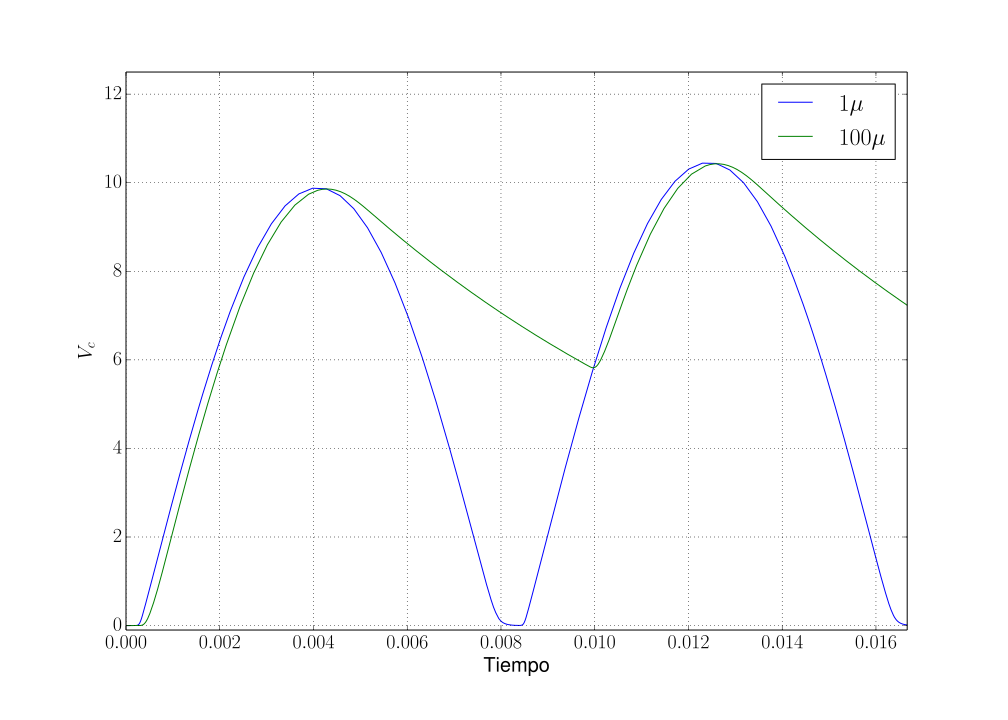
\includegraphics[width=0.5\textwidth]{images/filtrofuentedc.png}
\caption{Salida Filtro}
\end{figure}

El comportamiento mostrado en la figura anterios se puede considerar el
voltaje de salida (grafica verde) $V_{c}$ tiene un componente de DC
(offset) más un componente de AC llamado voltaje de rizo.

Se tiene que el voltaje máximo del capacitor $V_{m}$ es:

\begin{equation}\label{eq:vm}
V_{m}=V_{s}-2V_{d}
\end{equation}

el voltaje mínimo $V_{l}$ es determinado por la expresión:

\begin{equation}\label{eq:vl}
V_{l}=V_{m}e^{\frac{-T_{d}}{RC}}
\end{equation}

a partir de las expresiones \eqref{eq:vm} y \eqref{eq:vl} se de define
el volateje de rizo como:

\begin{equation}\label{eq:vr}
V_{r}=V_{m}-V_{l}=V_{m}-V_{m}e^{\frac{-T_{d}}{RC}}=V_{m}(1-e^{\frac{-T_{d}}{RC}})
\end{equation}

la expresión \eqref{eq:vr} es una ecuación trasendente por lo que no
tiene solución analitica, por lo que para obtener una solución
aproximada se utiliza la expansión en series de Taylor de la siguiente
manera:

\begin{equation}\label{eq:taylorexp}
e^{\frac{-T_{d}}{RC}}\approx 1-\frac{T_{d}}{RC}
\end{equation}

sustituyendo \eqref{eq:taylorexp} en \eqref{eq:vr} se tiene

\begin{equation}\label{eq:vr2}
V_{r}\approx V_{m}\frac{T_{d}}{RC}
\end{equation}

Se tiene que el tiempo de descarga del capacitor $T_{d} \leq T$, por lo
que se considera que

\begin{equation}\label{eq:vr3}
V_{r} \leq V_{m}\frac{T}{RC}
\end{equation}


    \begin{Verbatim}[commandchars=\\\{\}]
Se encontraron 4 pasos en la simulacion
[  902.   916.   969.  1067.]
    \end{Verbatim}

    \begin{center}
    \adjustimage{max size={0.5\linewidth}{0.5\paperheight}}{Circuitos usando Diodos_files/Circuitos usando Diodos_21_1.png}
    \end{center}
    { \hspace*{\fill} \\}
    
    \section{Circuito Modulador de AM}\label{circuito-modulador-de-am}

Uno de los primeros circuitos usados en la electrónica fueron los
relacionados con las comunicaciones, siendo la
\href{http://es.wikipedia.org/wiki/Amplitud_modulada}{modulación en
amplitud} una de las primeras tecnicas utilizadas. Uno de los circuitos
teoricos más faciles de usar es el que se muestra acontinuación.

\begin{figure}[htbp]
\centering
\includegraphics{images/undiodoam.png}
\caption{Modulador AM con un diodo}
\end{figure}



    % Add a bibliography block to the postdoc
    
    
    
    \end{document}
